%\documentclass[handout]{beamer}
\documentclass[•]{beamer}
\usepackage[latin1]{inputenc}
\usepackage{amsmath}
\usetheme{Luebeck}
\setbeamertemplate{footline}[frame number] 
\setbeamertemplate{navigation symbols}{} 
\usepackage{graphicx}
\usepackage{caption}
\usepackage{subcaption}
\theoremstyle{remark}
\graphicspath{{plots/}{Figforpres/}}
%\setbeamerfont{caption}{size=\tiny}

%\usepackage{caption}
%\captionsetup{font=scriptsize,labelfont=scriptsize}

\title{Masters thesis: Impact of ATLAS phase II performance on a mono-jet analysis}
\subtitle{Half-time presentation}
\author{Patrik Hallsj\"{o}}
%\date{\today} 
\begin{document}
\begin{frame}
\titlepage
\end{frame}
\begin{frame}\frametitle{Brief introduction}
\begin{block}

This presentation serves to present what goals were set up and what progress has been made.
\end{block}
\end{frame}

\begin{frame}[allowframebreaks]
\tableofcontents
\end{frame}


\section{Research goals}
\begin{frame}[shrink=30]\frametitle{Goals}
\begin{itemize}
\item Implement a C++ programme that loops over the collisions inside the signal and background datasets.	 \textbf{Complete}
\item For each collision retrieve the relevant observables (variables used to	 extract the signal over the background) and apply "smearing functions" to emulate the effect of the high luminosity on the observables. \textbf{Complete}
\item For both signal and background datasets, compare observables before and after smearing. What observables are the least/most affected? \textbf{Complete}
\item Implement selection criteria that selects the signal collisions efficiently while reduces significantly the background. In a first step the selection criteria should be taken from existing studies. \textbf{Complete}
\item Selection criteria can be evaluated and compared with each other using a figure of merit Z, that measures the sensitivity of the experiment to the dark matter signal. Calculate Z for the given selection criteria before and after smearing. \textbf{Complete}
\item What is the effect of the high luminosity (smearing) on the value of Z?  \textbf{Work in progress}
\item Investigate other selection criteria and observables, to mitigate the effect of high luminosity. Use Z to rank different criteria after smearing.  \textbf{Work in progress}
\item Conclude on the effect of the high luminosity on the sensitivity for dark matter and possible ways to mitigate its effects using alternative observables and selection criteria. \textbf{Work in progress}
\end{itemize}
\end{frame}

\section{Theoretical Background}
\begin{frame}[shrink=10]\frametitle{Dark matter}
\begin{block}

Dark matter is the name given to the solution to the discrepancies of galactic rotations. It is not known what it is only that it should not interact electromagnetically, (dark) and that it should interact through gravity (matter). 

It is experimentally shown that the  dark matter in the universe is mostly cold dark matter (high mass [GeV]). 

There are no candidates anywhere in the standard model that fulfils all three requirements. (Neutrinos could fulfil two.)
\end{block}
\end{frame}
\begin{frame}[shrink=10]\frametitle{Beyond the standard model: Supersymmetry}
\begin{block}

SUSY has several different possible candidates for dark matter. 
This will be expanded during the course of time.
\end{block}
\begin{figure}
%\fbox{
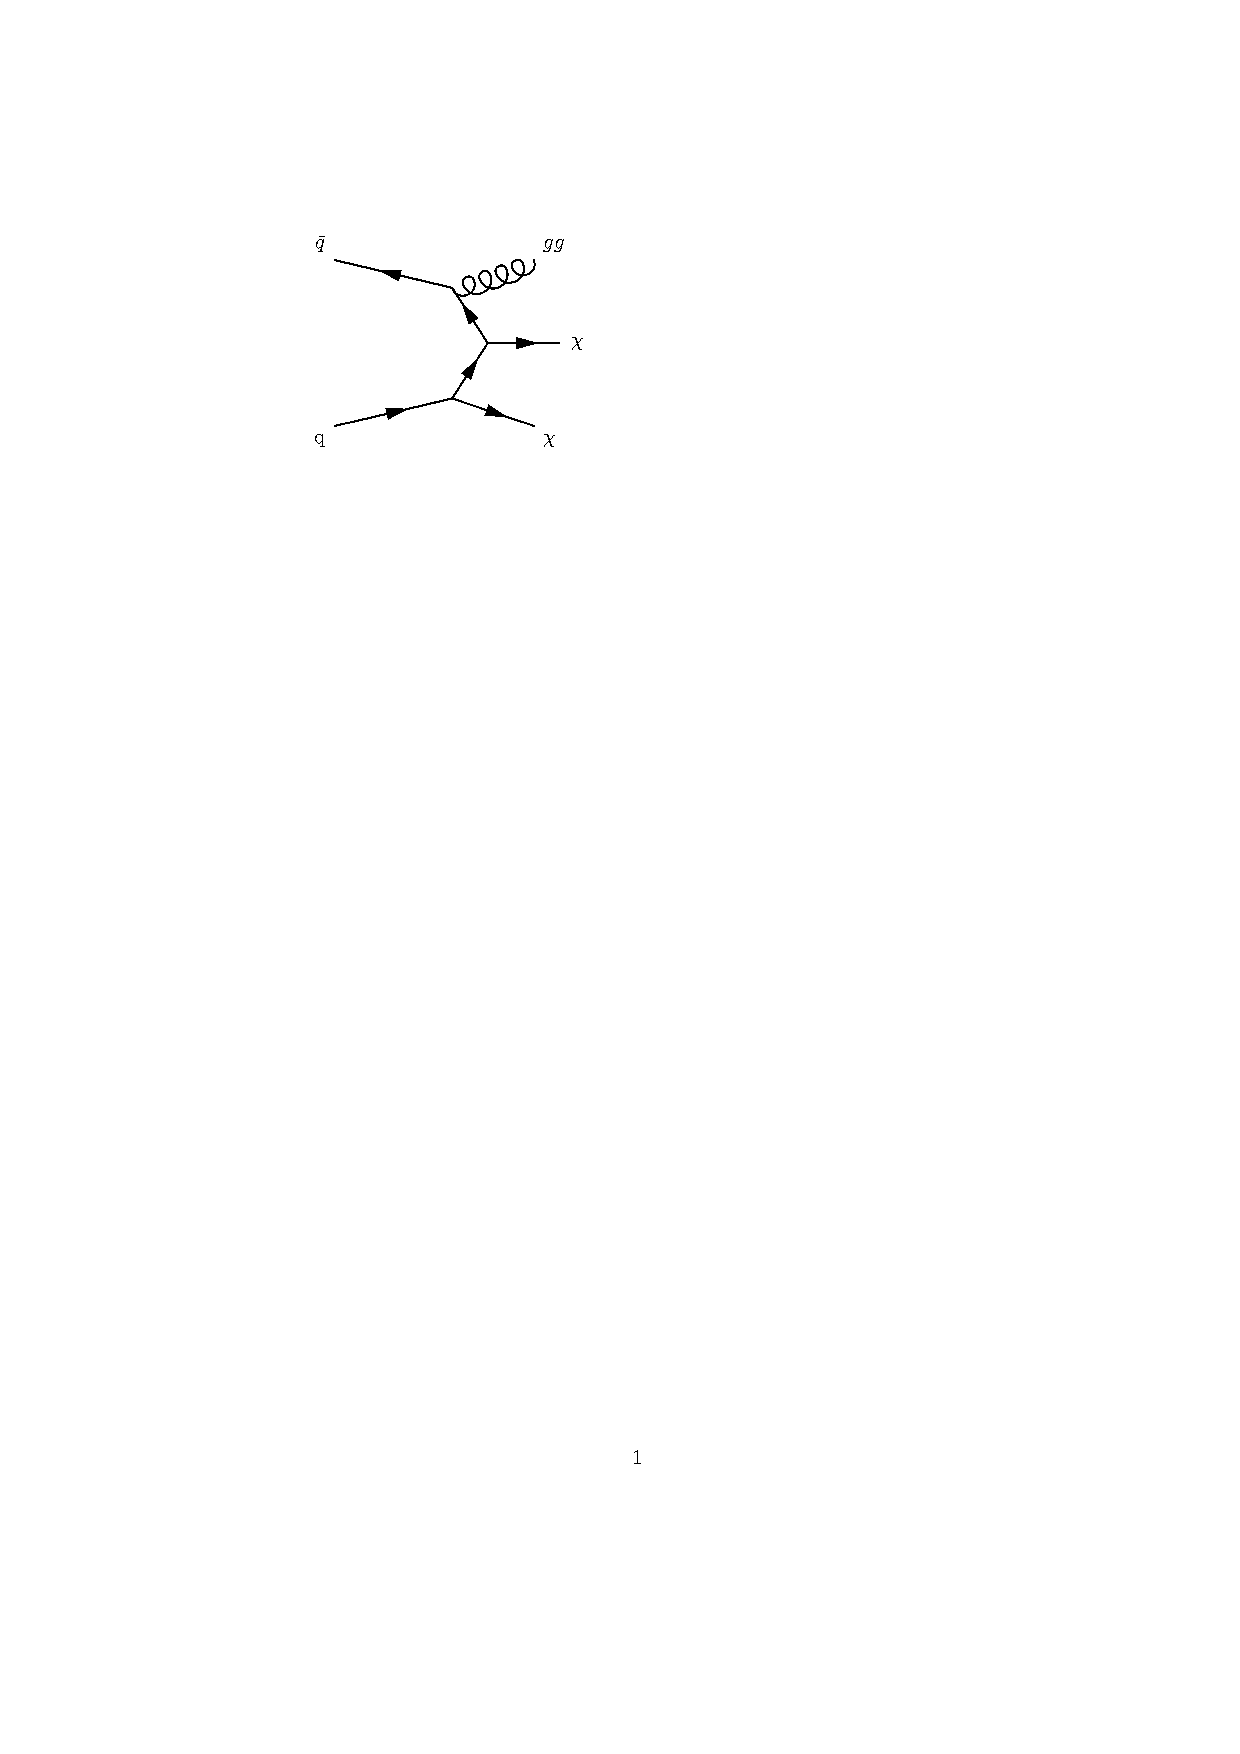
\includegraphics[trim=5cm 22cm 11cm 3.9cm,clip=true, width=0.45\textwidth]{dm.pdf}
%}
\end{figure}
\end{frame}

\begin{frame}\frametitle{Effective field theory}
\begin{itemize}
\item The WIMP (usually denoted $\chi$) is assumed as the only particle in addition to the standard model fields. 
\item $\chi$ will be assumed odd under some $Z_2$ symmetry. This means that an even number of $\chi$ must be in every coupling. 
\item It is assumed that the whatever mediator exists is heavier that the WIMPS, meaning that their interactions are in higher order terms of the effective field theory and thus not included in the operators. 
\item For simplicity, the WIMPS are assumed to be SM singlets, thus invariant under SM gauge transformations, and the coupling to the Higgs boson is neglected.
\end{itemize}
\end{frame}
\begin{frame}[shrink=10]\frametitle{Effective field theory}
\begin{block}

The focus for the operators will be quark bilinear operators on the form $\bar{q}\Gamma q$ where $\Gamma$ is a 4 $\times$ 4 matrix of the complete set, 
\begin{equation*}
\Gamma = \left\lbrace 1,\gamma ^5,\gamma ^\mu,\gamma ^\mu \gamma ^5, \sigma ^{\mu \nu} \right\rbrace
\end{equation*}
This, together with the couplings to GG define an effective field theory of the interaction of singlet WIMPS with hadronic matter. It is a non-renormalizable field theory which will break down when the mediator mass close to the mass of the WIMP.
\begin{equation*}
m_\chi \leqslant 2\pi M_*
\end{equation*}
Where $m_\chi$ is the mass of the WIMP and M$_*$ is the mass of the mediator. 
\end{block}
\end{frame}
\begin{frame}\frametitle{Effective field theory}
In this work, WIMPS are assumed to be Dirac fermions (half integer spin and is not its own antiparticle). 
\renewcommand{\arraystretch}{1.5} %Change height of tabel
\begin{table}[H]
\begin{center}
    \begin{tabular}{ | l | l | l | l |}
    \hline
    Name & Initial state & Type & Operator \\ \hline
  	D5 & qq & vector & $\frac{1}{M^2_*} \bar{\chi} \gamma^\mu \chi \bar{q} \gamma_\mu q$ \\ \hline

  	\end{tabular}

  	\caption{From {CERN-PH-EP-2012-210}}
  	\label{tab:operators}
  	  	\end{center}
    \end{table}
\renewcommand{\arraystretch}{1.0}  %Back to default
\end{frame}
\begin{frame}\frametitle{Search for WIMPS}
\begin{block}

One of the candidates for dark matter, the one of interest here, is a WIMP (Weakly Interactive Massive Particle). 

Through SUSY there are particle candidates. 

The idea of my research is to find limitations of the mass in the different models. As in the operators above.
\end{block}
\end{frame}
\begin{frame}\frametitle{Monte Carlo simulation}
\begin{block}

The simulated data is produced using a Monte Carlo simulation. The simulation only takes the interaction into account, no detectors. 

This is why in the thesis several "smearing" functions are used. These functions alter the data to simulate what will be detected when the pile-up has been taken into account.
\end{block}
\end{frame}
\section{Experimental overview}
\begin{frame}\frametitle{Coordinate system}
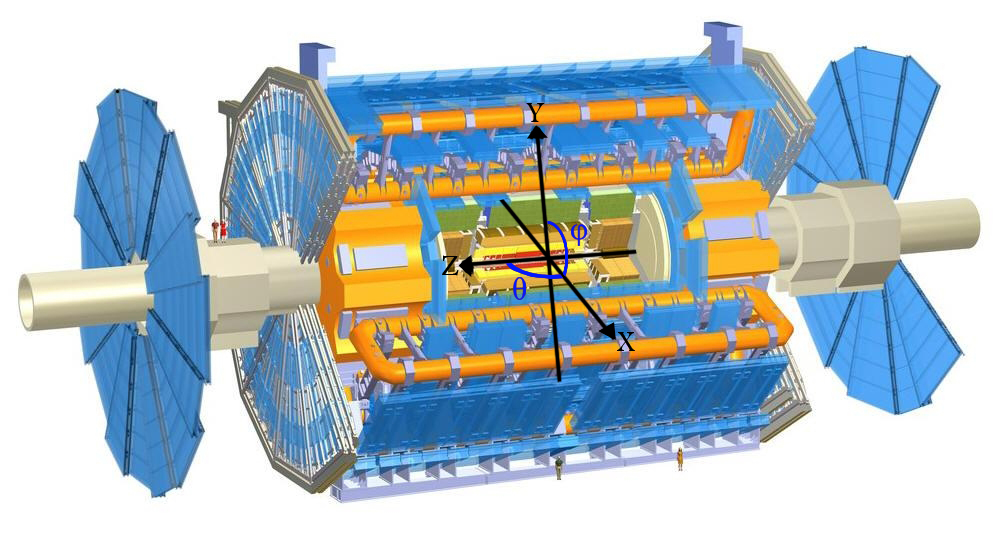
\includegraphics[scale=0.3]{particle_collider.jpg}
\end{frame}
\begin{frame}\frametitle{Jet and missing energy}
\begin{block}

In particle collisions, often jets are produced. These are showers of quarks or gluons that travel with high energy in a conform direction and interact during their time in the detector.

How does one find dark matter? 

If the detectors can not find it, look in the transversal missing energy (Mono-jet events). Can be comprised of neutrinos and exotic matter.

\end{block}
\end{frame}

\begin{frame}[shrink=10]\frametitle{Jet and missing energy}
\begin{block}

Missing energy refers to the modulus of the missing momenta. It is well known that in the transversal direction momenta before should be 0. 
\end{block}
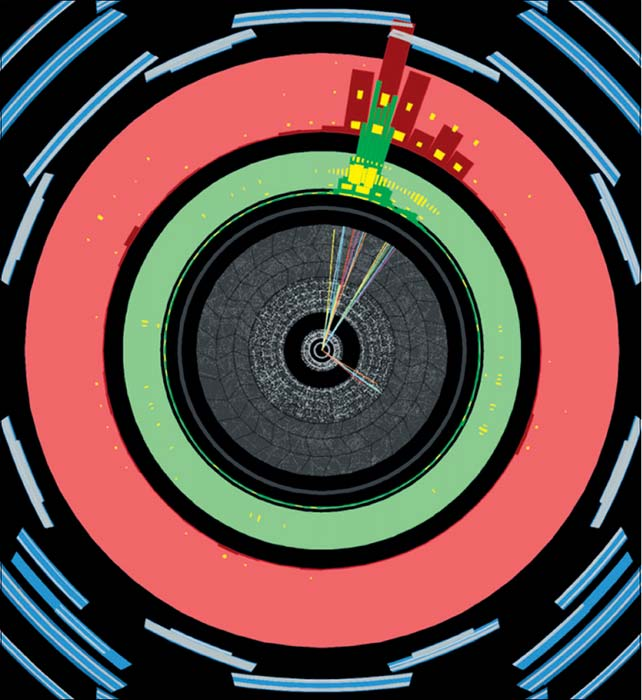
\includegraphics[scale=0.2]{monojet.jpg}


{\tiny image from \url{http://cerncourier.com/cws/article/cern/52017}}
\end{frame}
\begin{frame}



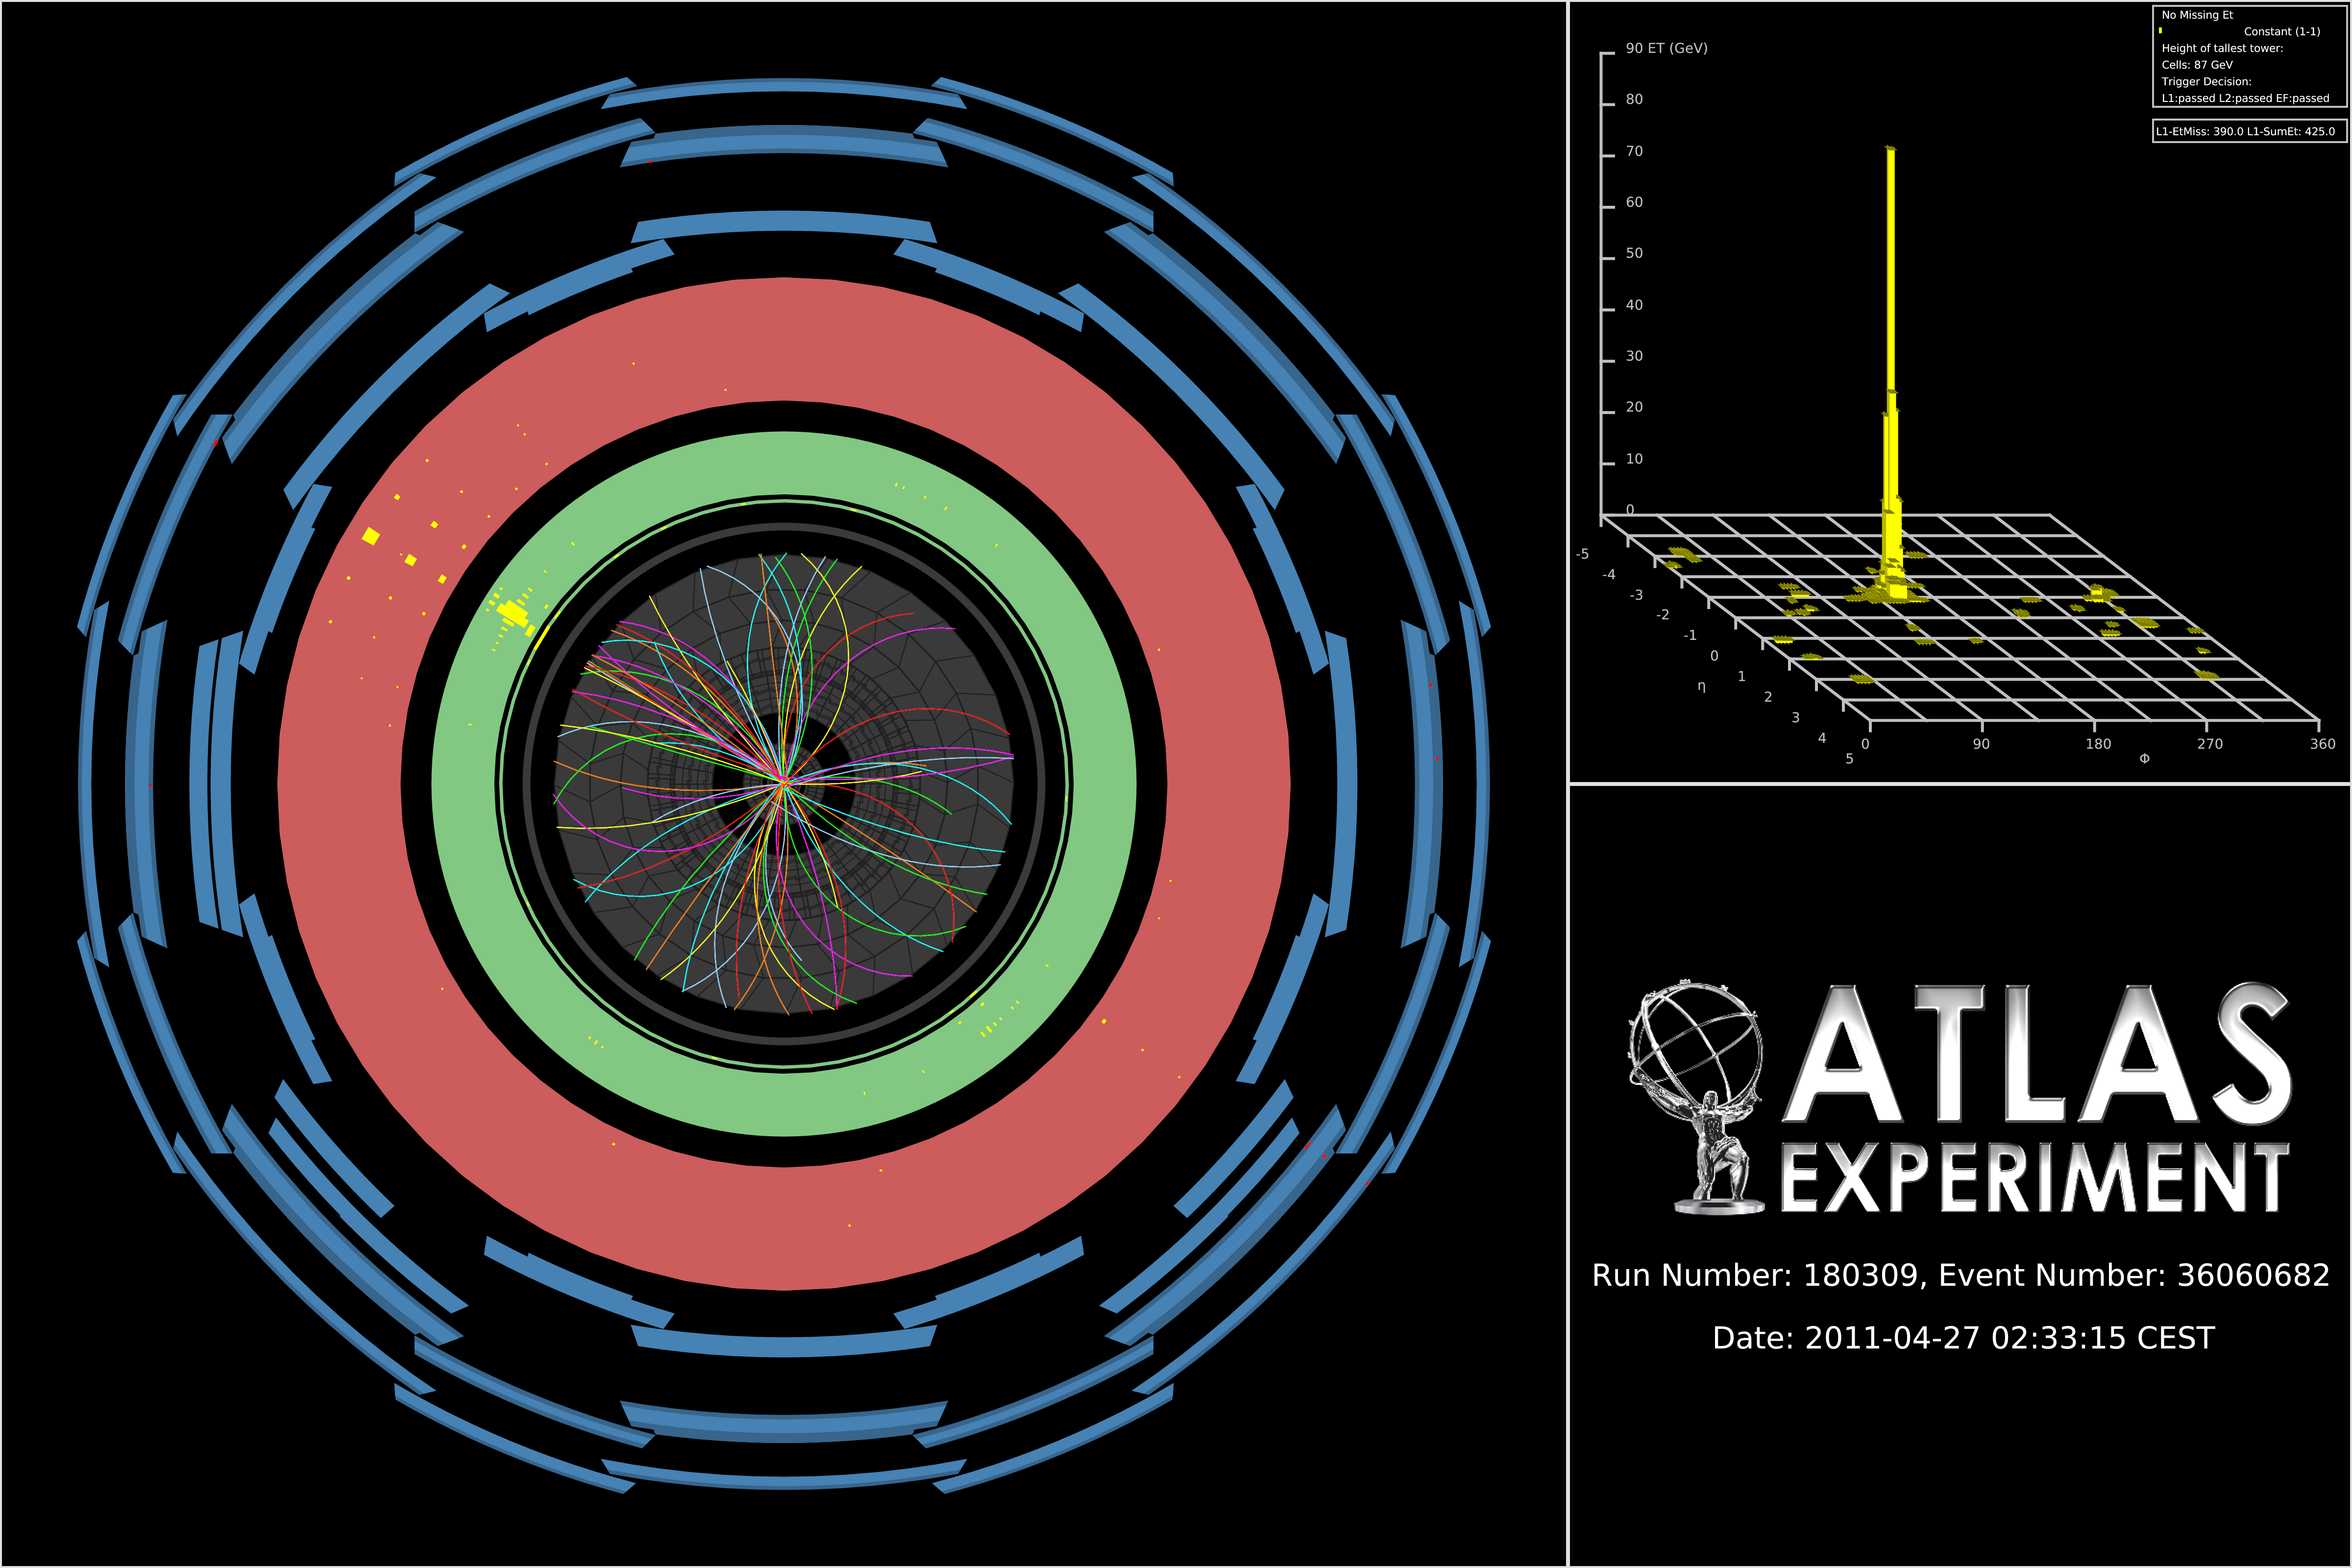
\includegraphics[scale=0.06]{monojetbig.png}


{\tiny \url{https://atlas.web.cern.ch/Atlas/GROUPS/PHYSICS/CONFNOTES/ATLAS-CONF-2011-096/fig_08.png}}


\end{frame}
\begin{frame}[allowframebreaks]\frametitle{Terminology}
\begin{itemize}
\item For two collinear intersecting particle beams the instantaneous luminosity is defined as:
\begin{equation}
l = \frac{fkN_1 N_2}{4\pi \sigma_x \sigma_y}
\end{equation} 
where $N_i$ are the number of particles in each of the bunches, f is the frequency at which the bunches collide , k the number of colliding bunches in each beam, and $\sigma_x$ ($\sigma_y$) is the horizontal (vertical) beam size at the interaction point. 

\item The expected number of events can be calculated by using the instantaneous luminosity through the following:
\begin{equation}
N=\sigma \int l dt := \sigma L
\end{equation}
where L is the luminosity and $\sigma$ is the cross section which is often measured in barn. 1 barn(b)$=10^{-24}$ cm$^2$. The luminosity is a measurement of total number of interactions that have occurred over time.

\item The cross section is defined through the integral of the differential cross section over the whole solid angle:
\begin{equation}
\sigma = \oint d\Omega \frac{d\sigma}{d\Omega}
\end{equation}
The cross section is therefore a measure of the effective surface area seen by the impinging particles, and as such is expressed in units of area. The cross section is proportional to the probability that an interaction will occur. It also provides a measure of the strength of the interaction between the scattered particle and the scattering center.

\end{itemize}


\end{frame}

\begin{frame}\frametitle{Phase II high luminosity upgrade}
\begin{block}

I am looking at the upgrade which will be done at CERN and will be completed around 2022-2023 and is denoted High Luminosity LHC Phase 2 upgrade. When this is running the following is expected:
\end{block}
\renewcommand{\arraystretch}{1.5} %Change height of tabel
\begin{table}[H]
\begin{center}
    \begin{tabular}{ | l | l | l |}
    \hline
    Entity & Expected & Last run (2012) \\ \hline
  	Luminosity & 1000-3000 fb$^{-1}$ & 20.8 fb$^{-1}$ \\ \hline
  	Pile-up & $\langle \mu \rangle=200$ & $\langle \mu \rangle=20.7$ \\ \hline
  	Center of mass energy & $\sqrt{s}=14$ TeV &  $\sqrt{s}=8$ TeV \\ \hline
  	\end{tabular}
  	
   	\end{center}
    \end{table}
    \renewcommand{\arraystretch}{1.0}  %Back to default

\end{frame}
\begin{frame}\frametitle{What have I done?}
\begin{block}

So far I have quickly gone over some theory, the question still remains, what have I done so far and what is left to do?

Most of what has been done so far is to set the foundation for the analysis work (which has just started). Hopefully the following will serve as a nice appetizer
\end{block}

\end{frame}
\section{Validation of smearing functions}
\begin{frame}\frametitle{Smearing}
\begin{block}

As discussed before, the MC simulation does not take the detectors or pile-up into account. This is done by "smearing" functions. 

One of the first steps in the project was to ensure that the given functions conformed to the letter of intent for the phase II HL upgrade.
\end{block}

\end{frame}
\begin{frame}\frametitle{Validation}
\begin{block}

\begin{itemize}
\item This is a part of a talk I gave at SU.
\item Emulate the ATLAS detector performance and the beam conditions of the Phase 2 LHC by smearing the Lorentz vectors of the truth data.
\item The expected response has been calculated and taken from: ATL-PHYS-PUB-2013-004
\item Below are figures that compare energies before and after the smearing. 
\end{itemize}
\end{block}
\end{frame}
\begin{frame}\frametitle{Processes simulated}
\begin{example}
The smearing functions affect the following, and data is taken from the following processes.
\begin{itemize}
\item Electron, W$\rightarrow e\nu$
\item Muon, W$\rightarrow \mu \nu$
\item $\gamma$, $\gamma$ + Jet sample.
\item Tau, W$\rightarrow \tau \nu$
\item Jets, Jet sample.
\item $E_T^{Miss}$, Z$\rightarrow \nu \nu$ + Jet sample
\end{itemize}
\end{example}
\end{frame}
\begin{frame}\frametitle{Processes simulated}
\begin{block}

The pile-up rate was fixed at 60 for all these validations, also to shorten the presentation only the electron was presented in full. 
\end{block}
\end{frame}
\begin{frame}[shrink=20]\frametitle{Electron}
\begin{block}

Here are all electrons paired with their smeared counterparts.
\end{block}
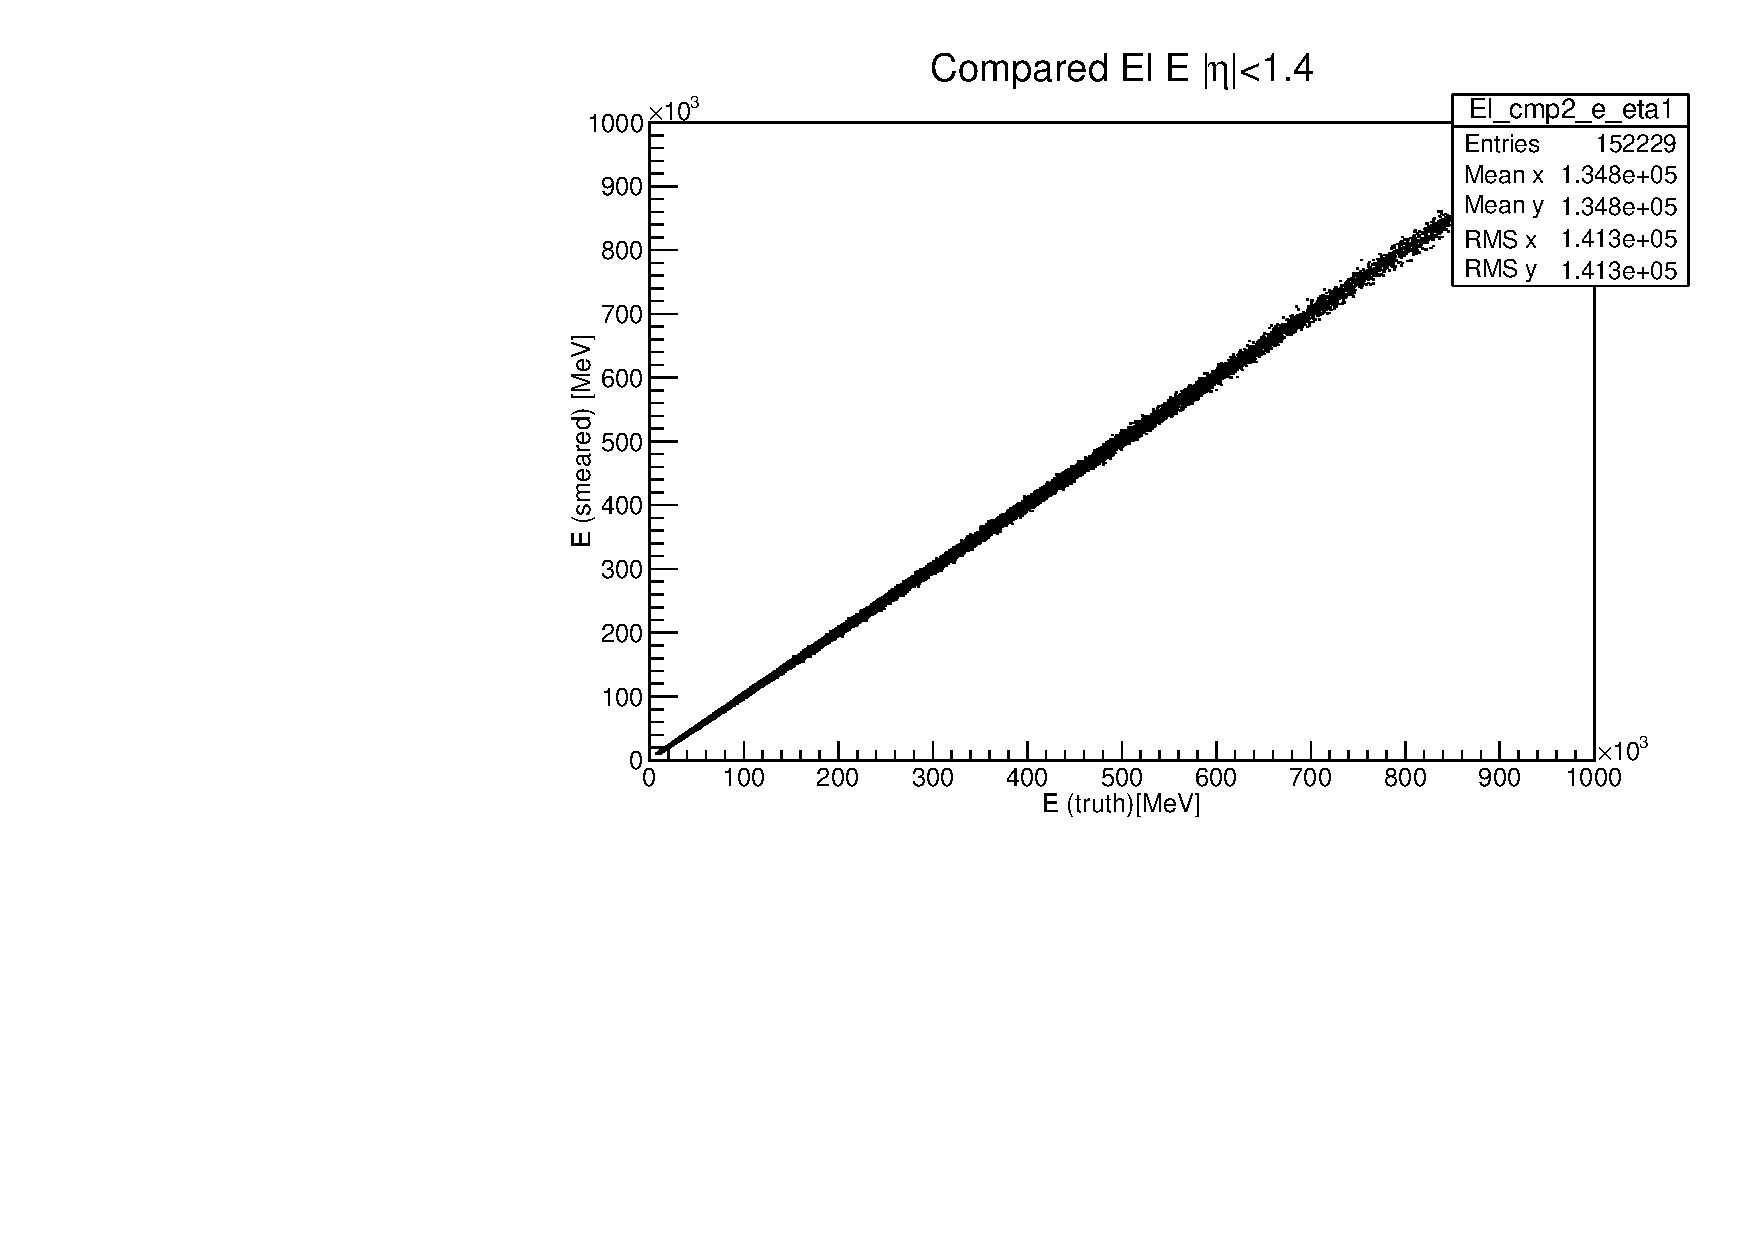
\includegraphics[scale=0.4]{Figforpres/eleta1plot.pdf}
\begin{block}

As expected, the smearing produces a widening line.
Where: $\eta = - \ln( \tan\frac{\theta}{2})$
\end{block}
\end{frame}

\begin{frame}\frametitle{Electron}
\begin{block}

\begin{itemize}
\item To emulate the fact that not all particles/jets are identified (efficiency), a random number generator is used to randomly throw away electrons that exist at the truth level.
%Only truth electrons that survive are smeared and studied.\\
\item Also, the code makes sure that only the data which is smeared is plotted against its unsmeared counterpart. 
\end{itemize}
\end{block}
\end{frame}
\begin{frame}[shrink=20]\frametitle{Electron}
\begin{block}

Taking a slice of truth around E=75 GeV. 
Taking here for $|\eta|<$ 1.4 and 1.4 $<|\eta|<$ 2.47 
\end{block}
\begin{figure}[tbp]
\centering
\begin{subfigure}[b]{0.4\textwidth}
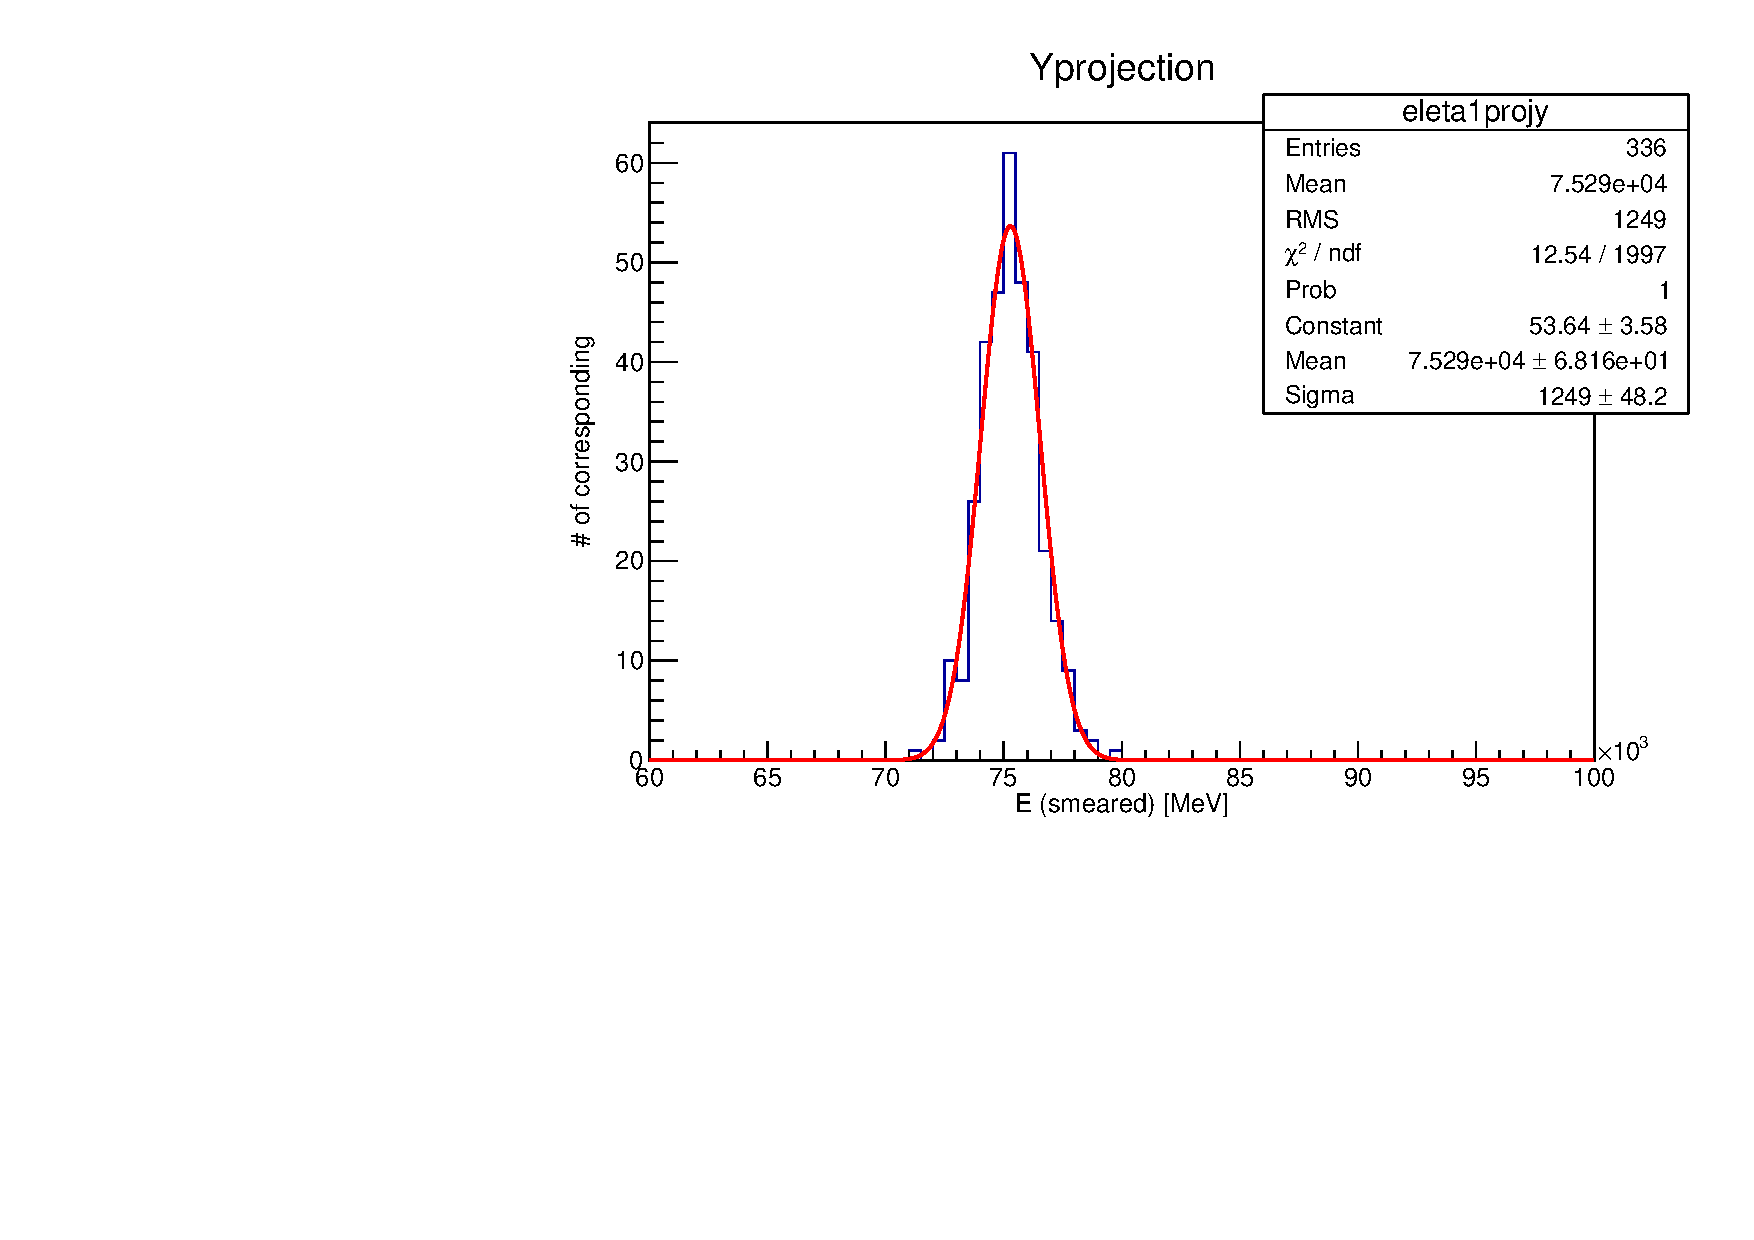
\includegraphics[width=\textwidth]{Figforpres/eleta1fill.pdf}
\end{subfigure}
\begin{subfigure}[b]{0.4\textwidth}
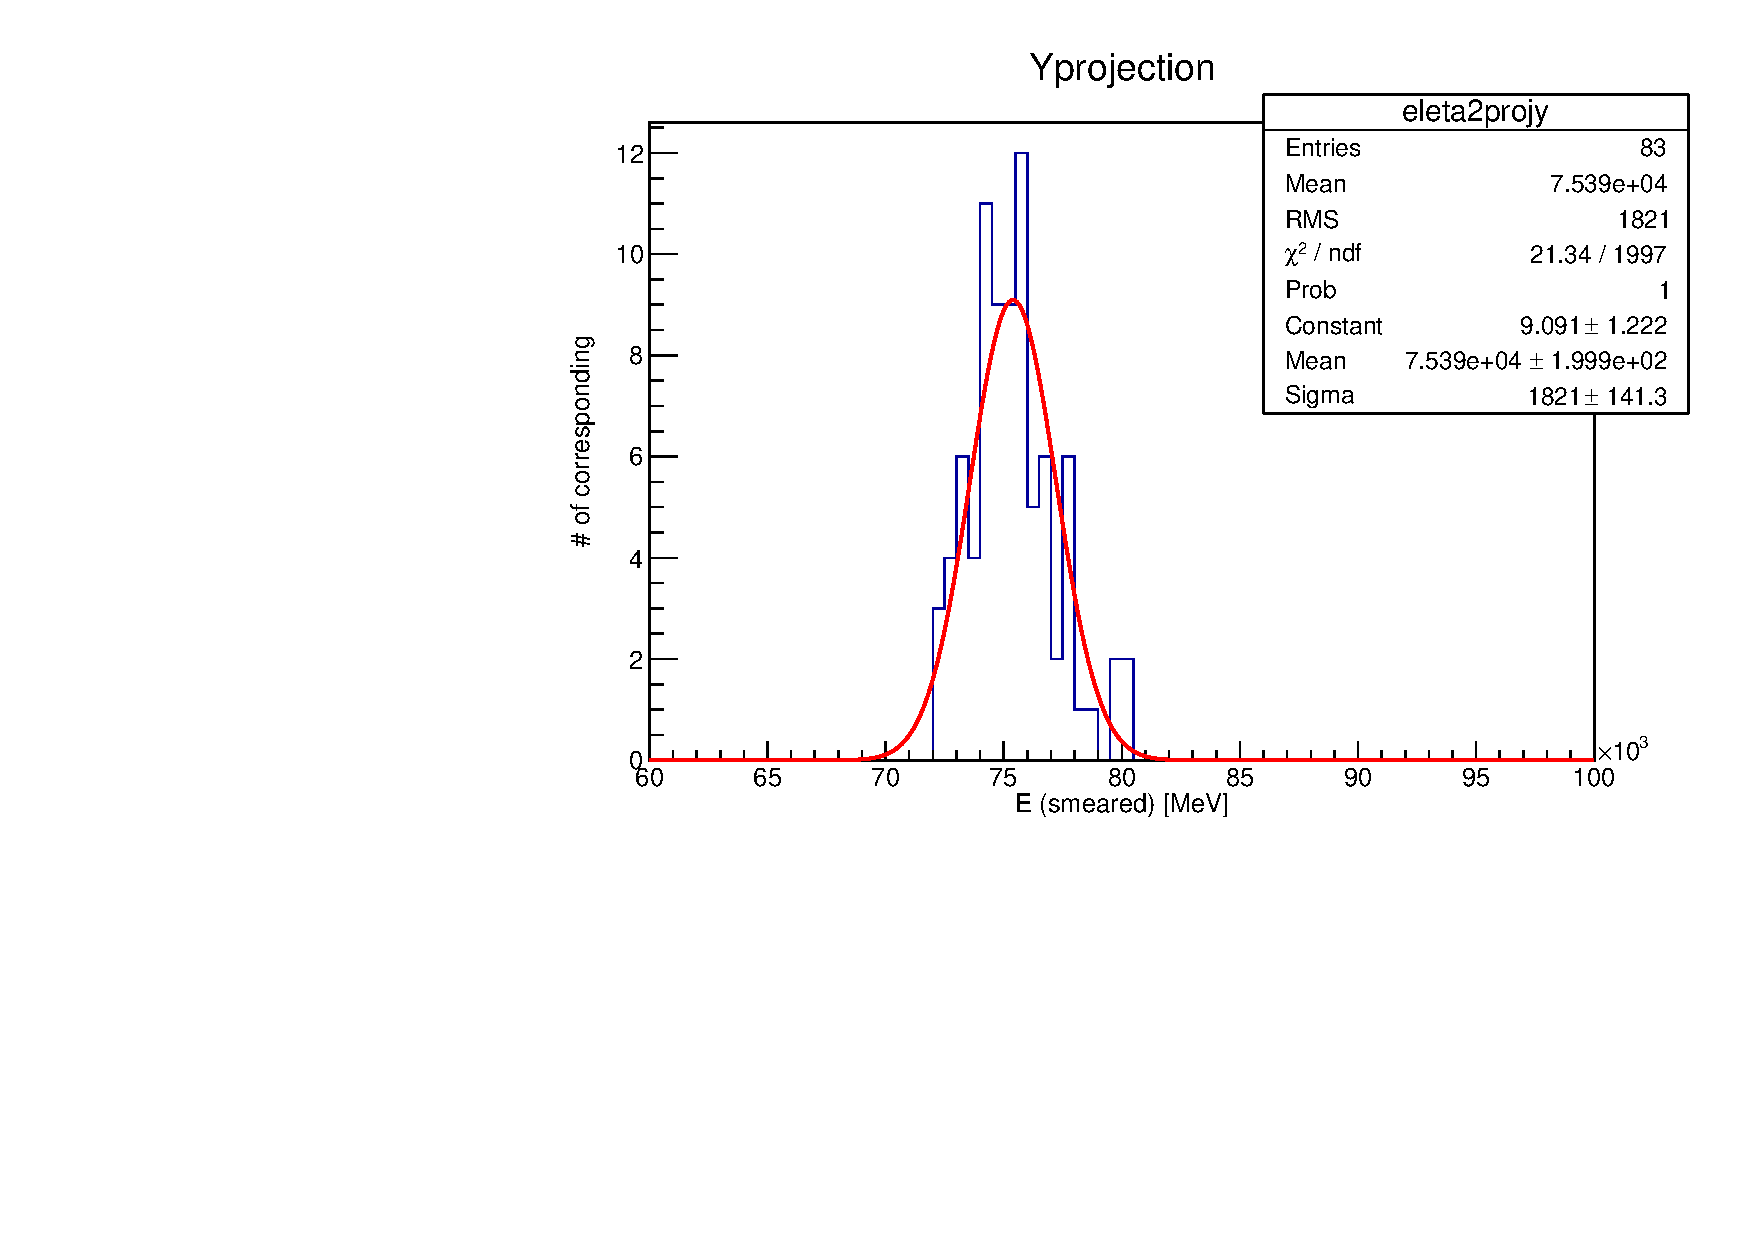
\includegraphics[width=\textwidth]{Figforpres/eleta2fill.pdf}
\end{subfigure}
\end{figure}
\begin{block}

$\sigma=0.3\oplus 0.1\sqrt{E(GeV)}\oplus 0.01E(GeV)$, $|\eta|<$ 1.4
$\sigma=0.3\oplus 0.15\sqrt{E(GeV)}\oplus 0.015E(GeV)$, 1.4 $<|\eta|<$ 2.47 
\end{block}
\end{frame}

\begin{frame}[shrink=20]\frametitle{Comparing sigma}
\begin{center}
    \begin{tabular}{ | l | l | l | l |}
    \hline
    Entity & Expected $\sigma$ MeV & $\sigma$ MeV & significance \\ \hline
    Electron, low eta 75GeV & 1184 & 1249 & 1.35$\sigma$ \\ \hline
    Electron high eta 75GeV & 1744 & 1821 & 0.5$\sigma$ \\ \hline
    Muon low eta 75GeV & 1497 & 1190 & 2.8$\sigma$ \\ \hline
    Muon high eta 75GeV & 1593 & 1707 & 2.5$\sigma$ \\ \hline
   	$\gamma$ low eta 75GeV & 1184 & 1189 & 0.14$\sigma$ \\ \hline
    $\gamma$ high eta 75GeV & 1744 & 1802 & 1.5$\sigma$ \\ \hline
    $\tau$ 150GeV & 10339 & 10899 & $1.0\sigma$ \\ \hline
    	Jet low eta 100GeV & 11598 & 11397 & 0.6$\sigma$ \\ \hline
    Jet low mid eta 100GeV & 11935 & 11509 & 0.8$\sigma$ \\ \hline
    Jet high mid eta 100GeV & 10944 & 11291 & 1.1$\sigma$ \\ \hline
    Jet high eta 100GeV& 13500 & 16611 & 2$\sigma$ \\ \hline
      $E^{miss}_X$ 750GeV & 48448 & 45201 & 2.0$\sigma$ \\ \hline
       $E^{miss}_Y$ 750GeV & 48448 & 42690 & 2.3$\sigma$ \\ \hline
    \end{tabular}
\end{center}
\end{frame}
\begin{frame}\frametitle{Concerns}
\begin{block}

\begin{itemize}

\item Looking at the data and comparing to expected results one sees some discrepancies. 
\item The two main sources of errors are: small amount of statistics (smaller $\sigma$) and the error calculations in ROOT (programming language used).
\end{itemize}
\end{block}
\end{frame}

\section{Evaluating dark matter signals}
\begin{frame}\frametitle{Signal to background ratio}
\begin{block}

This is still a work in progress. All pieces are in place, what is needed is time to analyse all the signals from the models and to see which ones are viable.
\end{block}
\end{frame}
\begin{frame}\frametitle{Figure of merit}
\begin{block}

The figure of merit used is the p-value instead of previously declared z-value. The difference is that the p-value gives the percentage of probability that the signal is masked by statistical variations in the background where as the z-value gives this value in terms of $\sigma$ (Standard deviations).
This will be discussed more in the report when more work on this has been done.
\end{block}
\end{frame}
\begin{frame}[shrink=45]\frametitle{A sample figure of signal/background}
\begin{block}

Signal to background diagram of a model where: we assume WIMP pairs , with a light vector mediator. 
\end{block}
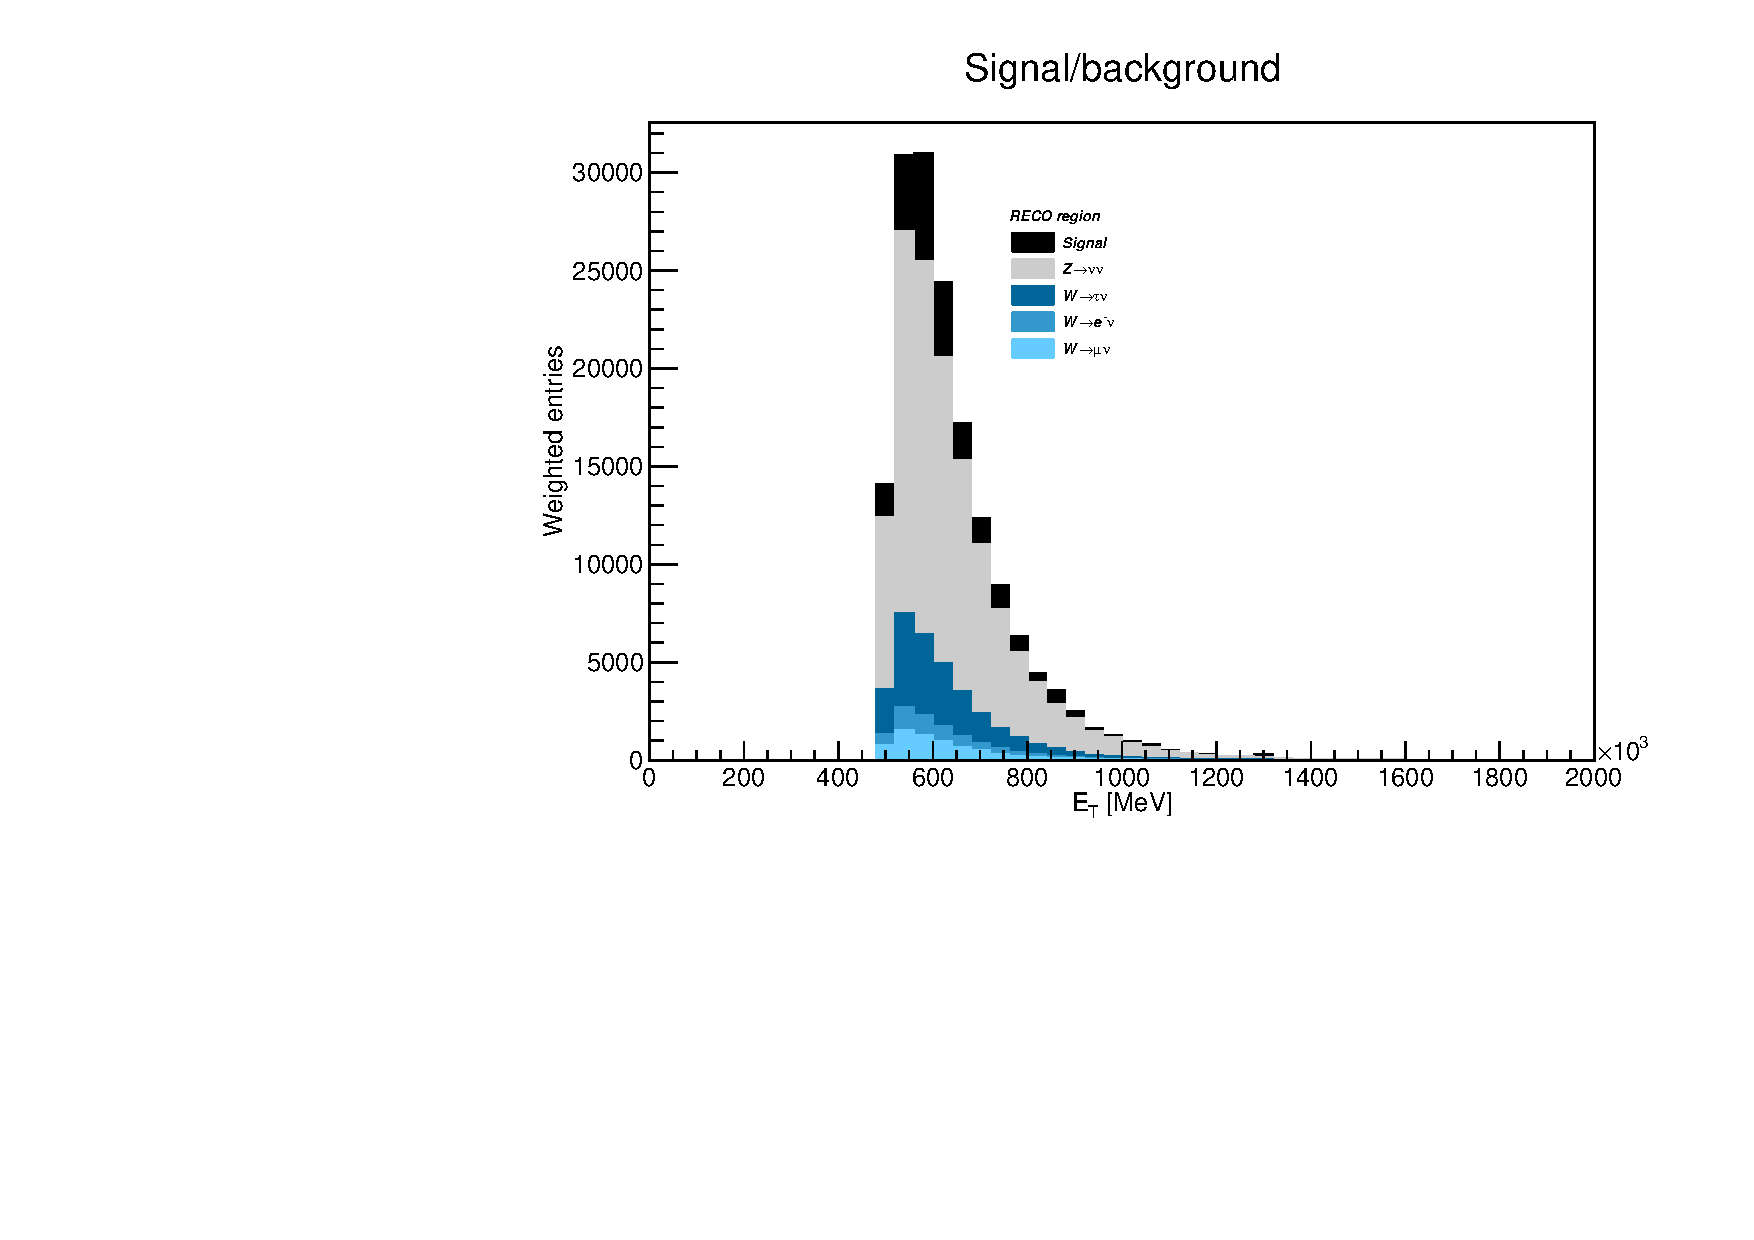
\includegraphics[scale=0.8]{signalbackgroundex.pdf}
\end{frame}
\section{Remaining work}
\begin{frame}\frametitle{Remaining work}
\begin{block}

\begin{itemize}
\item Evaluate different simulated signals for different WIMP candidates using the p-value and see how they are affected by pile-up.
\item See how the effect varies depending on signal region and observables.
\item Conclude which models are most viable and in which regions.
\item Finalize the report.
\end{itemize}
\end{block}
\end{frame}

\begin{frame}\frametitle{Thank you}
\begin{block}

Thank you for your attention.
\end{block}
\end{frame}

\begin{frame}[noframenumbering]\frametitle{Backup}
\end{frame}


\end{document}
